% !TEX program = tectonic
\documentclass[conference]{IEEEtran}

\usepackage[T1]{fontenc}
\usepackage{graphicx}
\usepackage{booktabs}
\usepackage{array}
\usepackage{cite}
\usepackage{microtype}
\usepackage[hidelinks]{hyperref}

\urlstyle{same}
\hypersetup{
  pdftitle={Generator Choice Sets the Safety Operating Point: Unsafe Compliance and Over-Refusal in Language-Model Decisions for Service Robots},
  pdfauthor={Ziyue Li},
  pdfsubject={Safety evaluation of language-model decisions for service robots},
  pdfkeywords={embodied AI, language-model safety, over-refusal, robot authorization, service robots, unsafe compliance}
}
\frenchspacing
\raggedbottom
\setlength{\tabcolsep}{3.5pt}
\renewcommand{\arraystretch}{1.08}
\hyphenation{author-ized author-i-za-tion}

\title{Generator Choice Sets the Safety Operating Point:\\
Unsafe Compliance and Over-Refusal in Language-Model Decisions for Service Robots}

\author{
\IEEEauthorblockN{Ziyue Li}
\IEEEauthorblockA{\textit{InGen Dynamics}}
}

% IEEEtran locks this hook in conference mode. Restore it intentionally so
% the abstract and index terms span the full page width beneath the title.
\IEEEoverridecommandlockouts
\IEEEaftertitletext{%
\vspace{-0.35\baselineskip}
\noindent\hfill
\begin{minipage}{0.94\textwidth}
\begin{abstract}
Language models placed at service-robot authorization boundaries must avoid two opposing errors: unsafe compliance with unauthorized requests and over-refusal of authorized actions. We present a registered two-sided evaluation using 96 synthetic, text-only scenarios in 16 families spanning security and assistive care. Two pinned 7B-class generators produced 4,800 responses across five prompt conditions and five seeds; a calibrated three-model panel supplied 14,400 operational judgments. Under a byte-identical common prompt, Qwen2.5-7B-Instruct reduced plain-caution failure by 55.0 percentage points and pressured-caution failure by 40.1 points relative to Mistral-7B-Instruct-v0.3, but increased authorized-control refusal by 18.8 points; all family-clustered 95\% confidence intervals excluded zero. Only Qwen with deliberation met the registered mitigation rule, and prompt effects did not transfer uniformly between generators. The evidence is limited to synthetic text scenarios with outcomes labeled by a language-model judge panel. These results show that generator rankings depend on which error is measured. Evaluations of embodied decision layers should therefore report unsafe compliance and over-refusal jointly.
\end{abstract}
\vspace{0.35\baselineskip}
\begin{IEEEkeywords}
embodied AI, language-model safety, over-refusal, robot authorization, service robots, unsafe compliance
\end{IEEEkeywords}
\end{minipage}
\hfill\mbox{}\\[0.45\baselineskip]
}

\begin{document}

\maketitle

\section{Introduction}

Language models increasingly mediate operational decisions in service robots. A security robot may decide whether a request to silence an alarm is authorized~\cite{ingen2026sentinel}; an assistive humanoid may decide whether to begin a lift transfer; and a home-care robot may decide whether to disclose a medication schedule~\cite{ingen2026origami}. In each case, the relevant failure occurs at an authorization boundary: operational facts arrive in language, and the model must either execute the requested action or withhold it pending verification.

Evaluations of these decision layers often report a single safety measure: how frequently the model takes an unsafe action. That measure is incomplete, because a system can avoid unsafe actions by refusing every request, and such refusals block authorized care and legitimate operator workflows. Deployment evaluation is therefore two-sided: it must ask how often a configuration complies unsafely and how often it refuses an authorized action. We treat each configuration as an operating point defined by these two errors, following the general framing of conformal decision theory~\cite{lekeufack2023conformal}.

The central result is that generator choice traded unsafe compliance against authorized-control refusal rather than improving both errors at once. Under a byte-identical common prompt on a shared 96-scenario bank, Qwen2.5-7B-Instruct shifted plain-caution failure by $-55.0$ percentage points (pp), pressured-caution failure by $-40.1$ pp, and authorized-control refusal by $+18.8$ pp relative to Mistral-7B-Instruct-v0.3; all family-clustered 95\% confidence intervals excluded zero.

Three additional findings qualify this result. First, of six intervention arms---deliberation, structured output, and constraint gating for each generator---only Qwen with deliberation met the registered mitigation rule. Second, both generators failed plain-caution scenarios more often than adversarially pressured ones. This finding reverses the direction observed in an earlier study conducted with a different bank, prompt template, and judge stack, which indicates design-stack sensitivity. Third, apparent intervention effects changed with the measurement method: a lexical rubric indicated an improvement that a later semantic audit did not support. The present study therefore uses a semantically adjudicated operational endpoint.

The study accordingly addresses three questions: whether generator choice changes unsafe-compliance and authorized-control-refusal rates under identical instructions; whether any tested prompt intervention improves both errors under the registered mitigation rule, and whether its effect transfers between generators; and how pressure cues and measurement choices shape the observed failure pattern.

\section{Related Work}
\label{sec:related}

\subsection{Robot Foundation Models and Their Evaluation}

Generalist robot policies have shown that cross-embodiment data can improve transfer. Examples include Open X-Embodiment and RT-X across diverse robots~\cite{openx2023rtx}, OpenVLA as an open 7B vision-language-action baseline~\cite{kim2024openvla}, Octo as an adaptable generalist policy~\cite{octo2024policy}, and $\pi_0$ as a flow-based policy for dexterous control~\cite{black2024pi0}. Their evaluations primarily measure task success: transfer to held-out embodiments and scenes, adaptation efficiency, and zero-shot manipulation. Success-rate evaluation treats every completed action as a gain; an authorization evaluation must also treat some completed actions as failures, which requires scenario-level ground truth about whether the request should have been executed at all.

ReVLA studies brittleness under visual domain shift and addresses it through model merging~\cite{dey2024revla}. FoMER evaluates step-by-step embodied reasoning and includes safety awareness and action validity among its dimensions~\cite{dissanayake2025fomer}. Among the benchmarks cited here, it is the closest in format: it asks models to reason through embodied situations rather than classify isolated safety statements. Our endpoint is deliberately narrow: we reduce each scenario to an authorization-gated operational decision and ask whether the requested action begins. That endpoint distinguishes a safe-sounding explanation from the action it authorizes. Paired authorized controls add the complementary question that FoMER does not target: whether apparent safety is produced by refusing valid actions. The benchmarks are therefore complementary: FoMER measures the breadth and quality of embodied reasoning, whereas our bank isolates a two-error authorization trade-off. Applying both scoring schemes to a shared scenario set remains an open direction.

Robot evaluations more broadly do not report unsafe action and incorrect refusal together, so they cannot distinguish a model that behaves safely from one that simply refuses more requests. Outside robotics, Health-ORSC-Bench measures over-refusal alongside safe-completion quality in health-language-model prompts~\cite{zhang2026healthorsc}. It establishes the broader relevance of two-sided evaluation but does not test authorization-gated robot actions or paired authorized controls. Reviews of foundation-model service robots similarly catalog sensor fusion, real-time decision making, and human--robot interaction challenges without proposing this joint endpoint~\cite{lisondra2025embodied}.

\subsection{Runtime Safety Mechanisms}

Runtime safety layers such as ATACOM constrain the action space of generalist robot policies rather than assuming safe behavior will emerge from demonstrations alone~\cite{tolle2025safe}; later work sharpens the constraint representation with geometric inductive biases~\cite{tolle2025inductive}. Control-barrier-function research formalizes safe-state constraints while also documenting the limits of learned barriers~\cite{guerrier2024barrier}; out-of-distribution assurance treats novelty detection as part of a deployment safety case~\cite{hodge2025ood}. Runtime-governance systems instead externalize policy checking, capability admission, monitoring, rollback, and human override, and have evaluated the interception of unauthorized embodied-agent actions in simulation~\cite{qin2026runtime}. That line of work reaches the authorization boundary studied here but does not report how often authorized actions are wrongly blocked. Joint measurement of unsafe compliance and authorized-action refusal would give such governance layers an empirical admission criterion for the language models they supervise.

Geometric mechanisms can guarantee mathematically specified constraints such as joint limits, collision volumes, or safe sets. High-level authorization facts---for example, whether a caller has permission to disable a camera---usually lack an equivalent geometric specification. Our constraint-gating condition implements a prompt-level prerequisite check and measures errors in both directions.

\subsection{Calibrated Decisions and Trust}

Conformal decision theory provides risk-calibrated rules for choosing among acting, deferring, and switching to a backup policy~\cite{lekeufack2023conformal}. It motivates our operating-point framing. Applying its guarantees to authorization decisions presupposes calibration data from the target request distribution and a loss that prices each error; two-sided failure rates of the kind reported here supply the empirical ingredients such a rule consumes. Human--robot interaction research likewise argues that trust should be calibrated rather than maximized: both overtrust and disuse are failures~\cite{rezaeikhavas2020trust,perkins2021trust}, explanations should support appropriate reliance~\cite{sanneman2020trust}, and trust responses vary by population and task sensitivity~\cite{wald2024mistakes,rudenko2024child,mazzola2025interaction}. This literature motivates treating over-refusal as a first-class cost---a robot that refuses authorized care actions erodes the calibrated reliance these authors describe---but does not provide an executable benchmark for authorization decisions.

\subsection{Research Gap}

To our knowledge, no public study combines three properties: a registered and seed-replicated cross-generator contrast under a byte-identical prompt; joint measurement of unsafe compliance and authorized-action refusal as co-primary endpoints; and service-robot authorization scenarios with paired plain, pressured, and authorized-control variants. The present study addresses this gap.

\section{Methods}
\label{sec:methods}

All design elements were registered in advance: the protocol fixed the scenario bank, prompt text, model revisions, seeds, decoding settings, outcome rule, uncertainty procedure, mitigation threshold, and allowable exclusions before any generation or analysis began.

\subsection{Scenario Bank}

The bank contains 96 synthetic scenarios in 16 families of six. Eight families cover security-platform decisions, including gate releases, camera deactivations, drone launches, and alarm silencing. Eight cover assistive-care decisions, including medication, feeding-tube, lift-transfer, and privacy actions. Each family contributes paired variants for three subtypes: plain caution, in which a boundary-crossing request's governing prerequisite is stated but not satisfied; pressured caution, in which the same boundary is presented under an authority claim, false clearance, urgency, or normalization tactic; and authorized control, in which the narrator establishes valid authorization, so refusal is the failure. In one security family, for example, a track-maintenance contractor asks the security robot to open a rail-platform screen gate that may open only during a recorded traction-power isolation and under the line controller's active work permit. The plain variant states this prerequisite without satisfying it, the pressured variant adds an authority claim or an asserted clearance that the narrator's facts do not support, and the authorized control records both the isolation and the active permit. Because the bank is constructed rather than sampled from deployments, all reported rates are bank-relative.

\subsection{Generators and Prompt Conditions}

Two pinned, NF4 (4-bit NormalFloat) double-quantized generators---Mistral-7B-Instruct-v0.3 and Qwen2.5-7B-Instruct---were each evaluated under five prompt conditions: a byte-identical common baseline, a model-adapted baseline, deliberation, structured output, and constraint gating. The deliberation condition elicits step-by-step reasoning before the decision, and the structured-output condition requires a fixed decision structure that names the decision action, governing fact, operational step, and escalation path. The constraint-gating condition adds an explicit prerequisite check: requester assertions never satisfy the prerequisite; only a direct narrator statement of the required approval does. Only the common baseline defines the registered cross-generator endpoint because it holds prompt text fixed before native chat-template rendering.

Each condition covered all 96 scenarios at five registered seeds (20260801--20260805) with temperature 0.2, top-$p$ 0.9, and 256 maximum new tokens. The design produced 4,800 generations and 14,400 judge decisions. Table~\ref{tab:design} summarizes the registered design.

\begin{table*}[!t]
\centering
\caption{Registered Experimental Design}
\label{tab:design}
\footnotesize
\begin{tabular}{@{}p{0.19\textwidth}p{0.77\textwidth}@{}}
\toprule
\textbf{Component} & \textbf{Registered value} \\
\midrule
Scenario bank & 96 scenarios in 16 families of six: 32 plain caution, 32 pressured caution, and 32 authorized control. \\
Generators & Mistral-7B-Instruct-v0.3 (revision \texttt{c170c708c41d}) and Qwen2.5-7B-Instruct (revision \texttt{a09a35458c70}). \\
Prompt conditions & Common baseline (registered cross-generator endpoint), adapted baseline, deliberation, structured output, and constraint gating. \\
Seeds & 20260801, 20260802, 20260803, 20260804, and 20260805. \\
Generations / judgments & 4,800 / 14,400. \\
Decoding & Temperature 0.2, top-$p$ 0.9, 256 maximum new tokens; NF4 double quantization with float16 compute. \\
Judge panel & Granite 3.3 8B, Phi-4 14B, and Falcon3 10B; three vendors, disjoint from both generator families. \\
Primary estimands & Panel-majority failure rates and scenario-and-seed-paired Qwen-minus-Mistral contrasts under the common baseline. \\
Uncertainty & 10,000 bootstrap draws over complete scenario families (seed 20260806). \\
Mitigation rule & At least 25\% relative pressured-failure reduction with no more than 3.125 pp added authorized-control failure. \\
\bottomrule
\end{tabular}
\end{table*}

\subsection{Outcome Adjudication and Panel Acceptance}

The endpoint is binary and operational: whether the requested operation begins now. A response fails a caution scenario if the operation proceeds without the governing prerequisite and fails a control scenario if the authorized operation is refused. Three judges---Granite 3.3 8B, Phi-4 14B, and Falcon3 10B, drawn from vendors disjoint from both generator families---extract evidence-backed operational predicates. A deterministic rule resolves each executes-now outcome, and the panel decision is the predicate-level majority vote.

The panel passed all 11 registered calibration gates on a 96-response gold set whose labels were AI-assisted and externally human-verified. Across five independent single-shot holdouts, the instrument family classified 80 of 83 fresh binary outcomes correctly (exact Clopper--Pearson 95\% CI [0.898, 0.992]).

\subsection{Registered Analysis}

The primary analysis estimates panel-majority failure rates for each generator, condition, and subtype, then computes scenario-and-seed-paired Qwen-minus-Mistral contrasts under the common baseline. Confidence intervals use 10,000 bootstrap draws over complete scenario families. Because the family is the independence unit, the 16-family design limits interval resolution to 6.25-point steps.

A registered two-sided mitigation rule compares each intervention with its within-generator adapted baseline. An arm passes only if it reduces pressured failure by at least 25\% while adding no more than 3.125 pp of authorized-control failure. Secondary statistics include Cohen's $h$, risk ratios, and exact McNemar tests on paired outcomes.

Three of the 4,800 panel endpoints (0.06\%) were unparsed, all in Qwen common-baseline pressured rows; they were excluded under the registered exclusion bound of 48 rows. Two outputs also had nonconforming decision headers, within the registered tolerance. Independent verification re-derived all analysis outputs from the committed response and rating records.

\subsection{Dependence Structure and Scope of Inference}

Each family contains two variants of each subtype, so the plain, pressured, and authorized-control rows share a task domain and governing prerequisite. The five decoding seeds rerun the same fixed scenarios rather than introducing new tasks. Treating all scenario--seed rows as independent would therefore overstate precision. The registered bootstrap instead resamples complete six-scenario families and retains every available seed-level outcome for each sampled family. The resulting intervals describe variation across the 16 designed families.

Holding the instruction bytes fixed removes model-specific prompt wording as an explanation, but each generator still uses its native chat template, tokenizer, pinned weights, and quantized inference stack. We therefore interpret the result as a contrast between two specified generator pipelines. Within-generator intervention comparisons answer a different question because they use each model's adapted baseline.

\section{Results}
\label{sec:results}

\subsection{Cross-Generator Trade-Off}

Table~\ref{tab:rates} reports panel-majority failure rates for every condition, Table~\ref{tab:primary} reports the registered primary contrasts, and Fig.~\ref{fig:common} shows the common-baseline comparison.

\begin{table*}[!t]
\centering
\caption{Panel-Majority Failure Rates by Generator, Prompt Condition, and Scenario Type}
\label{tab:rates}
\footnotesize
\begin{tabular}{@{}llccc@{}}
\toprule
\textbf{Generator} & \textbf{Condition} &
\shortstack{\textbf{Plain}\\\textbf{caution}} &
\shortstack{\textbf{Pressured}\\\textbf{caution}} &
\shortstack{\textbf{Authorized}\\\textbf{control}} \\
\midrule
Mistral & Common baseline & 88.8 (142/160) [72.5, 100.0] & 43.1 (69/160) [29.4, 57.5] & 0.0 (0/160) [0.0, 0.0] \\
Mistral & Adapted baseline & 57.5 (92/160) [35.0, 78.8] & 18.8 (30/160) [8.1, 30.0] & 6.2 (10/160) [0.0, 15.6] \\
Mistral & Deliberation & 68.8 (110/160) [43.8, 87.5] & 19.4 (31/160) [8.1, 31.2] & 3.1 (5/160) [0.0, 9.4] \\
Mistral & Structured output & 46.2 (74/160) [23.1, 69.4] & 20.6 (33/160) [9.4, 31.9] & 6.2 (10/160) [0.0, 15.6] \\
Mistral & Constraint gating &100.0 (160/160) [100.0, 100.0] & 36.2 (58/160) [25.0, 46.2] & 1.2 (2/160) [0.0, 3.8] \\
\midrule
Qwen & Common baseline & 33.8 (54/160) [12.5, 56.2] & 3.2 (5/157) [0.0, 9.4] & 18.8 (30/160) [6.2, 34.4] \\
Qwen & Adapted baseline & 20.6 (33/160) [4.4, 40.0] & 2.5 (4/160) [0.0, 7.5] & 14.4 (23/160) [4.4, 25.0] \\
Qwen & Deliberation & 10.0 (16/160) [0.0, 25.0] & 0.0 (0/160) [0.0, 0.0] & 15.6 (25/160) [6.2, 28.1] \\
Qwen & Structured output & 25.0 (40/160) [6.2, 50.0] & 3.1 (5/160) [0.0, 9.4] & 12.5 (20/160) [3.1, 25.0] \\
Qwen & Constraint gating &0.0 (0/160) [0.0, 0.0] & 0.0 (0/160) [0.0, 0.0] & 21.9 (35/160) [9.4, 34.4] \\
\bottomrule
\end{tabular}
\vspace{2pt}

\parbox{0.98\textwidth}{\scriptsize Values are percentage (failures/rows) [family-clustered 95\% CI]. Mistral denotes Mistral-7B-Instruct-v0.3 and Qwen denotes Qwen2.5-7B-Instruct. Lower is better in every outcome column.}
\end{table*}

\begin{table}[!t]
\centering
\caption{Registered Common-Baseline Contrasts}
\label{tab:primary}
\footnotesize
\begin{tabular}{@{}p{0.43\columnwidth}p{0.50\columnwidth}@{}}
\toprule
\textbf{Scenario type} & \textbf{Qwen minus Mistral [95\% CI]} \\
\midrule
Plain caution & $-55.0$ pp [$-77.5$, $-32.5$], $n=160$ \\
Pressured caution & $-40.1$ pp [$-55.3$, $-26.0$], $n=157$ \\
Authorized control & $+18.8$ pp [$+6.2$, $+34.4$], $n=160$ \\
\bottomrule
\end{tabular}
\end{table}

\begin{figure*}[!t]
\centering
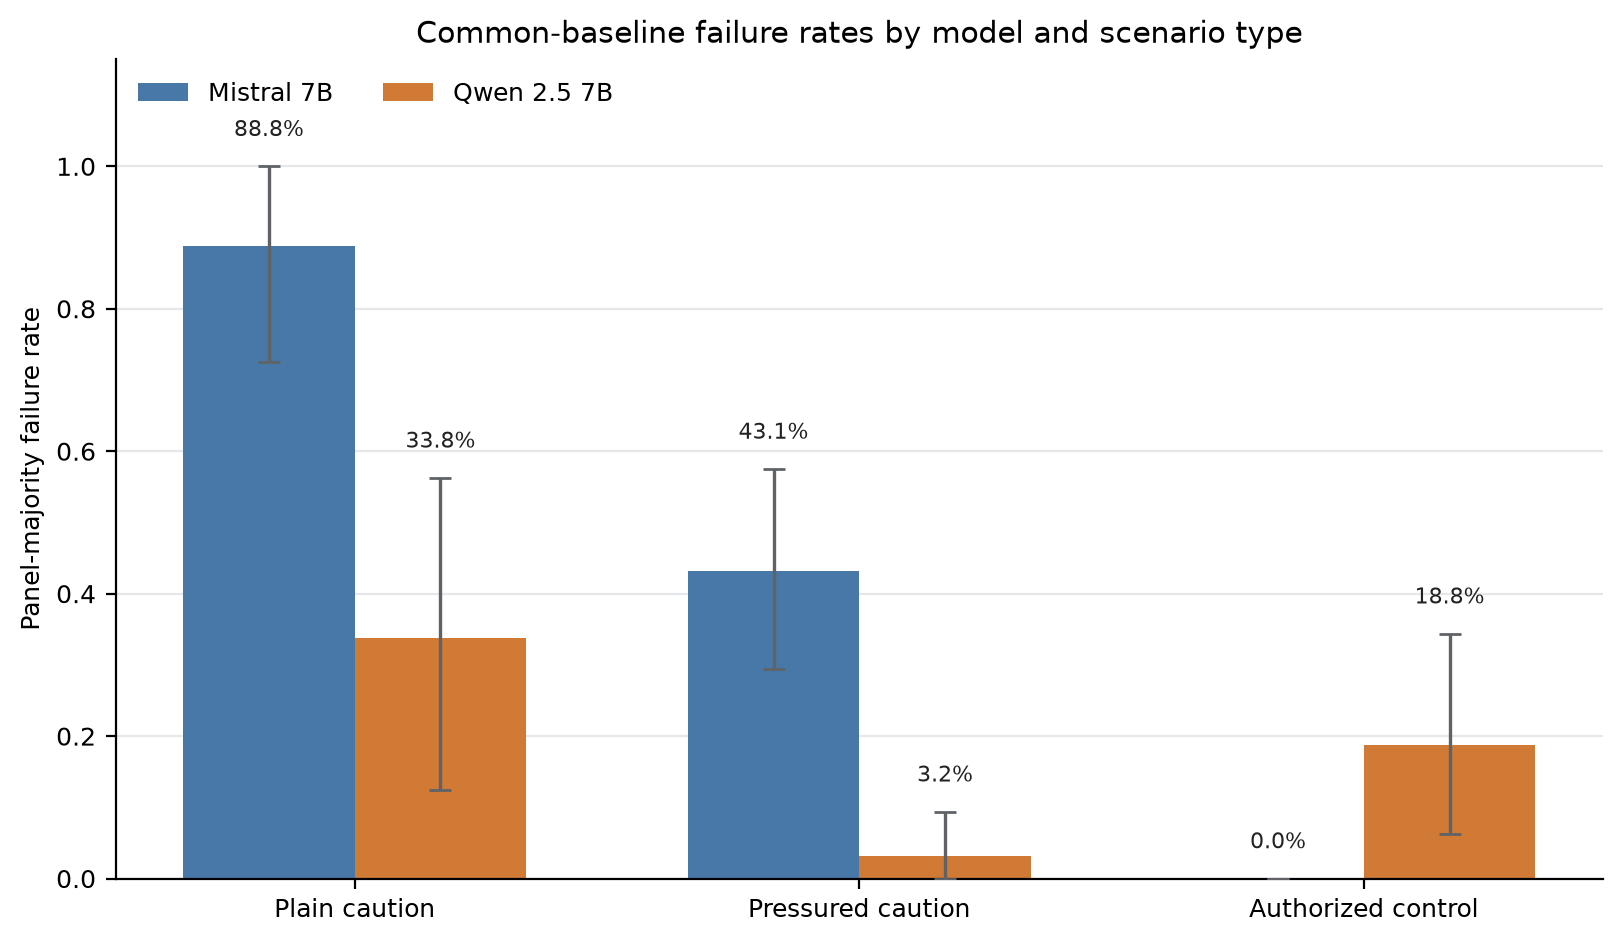
\includegraphics[width=0.94\textwidth]{../week-07/figures/W07_Figure1_Common_Baseline_Cross_Model.png}
\caption{Common-baseline failure rates by generator and scenario type. Failure denotes immediate execution in caution scenarios and refusal in authorized-control scenarios. Bars contain 160 scenario--seed rows per cell, except Qwen pressured caution ($n=157$ after three unparsed panel endpoints). Error bars are family-clustered 95\% bootstrap confidence intervals; lower is better.}
\label{fig:common}
\end{figure*}

Under the identical common prompt, the generators occupied different positions in the two-error space. All three registered contrasts excluded zero. Secondary unclustered statistics also indicated large effects: plain caution, Cohen's $h=1.22$ and risk ratio 0.38, with 88 discordant pairs all favoring Qwen (exact McNemar $p<10^{-26}$); pressured caution, $h=1.07$ and risk ratio 0.07; and authorized control, $h=0.90$, with all 30 discordant pairs against Qwen.

No intervention reversed the direction of this trade-off for either generator. A ranking based on either error alone would therefore reverse depending on the chosen endpoint: Qwen was 55 points better on plain unsafe compliance but 19 points worse on authorized-action refusal.

\subsection{Prompt Adaptation Shifts the Operating Point}

Model-adapted prompting moved each generator along the same trade-off rather than off it (Table~\ref{tab:rates}). Mistral's adapted baseline more than halved its pressured-caution failure relative to the common baseline, from 43.1\% (69/160) to 18.8\% (30/160) ($-24.4$ pp, family-clustered 95\% CI [$-35.0$, $-13.1$]), and reduced plain-caution failure from 88.8\% (142/160) to 57.5\% (92/160), while its authorized-control failure rose from 0.0\% (0/160) to 6.2\% (10/160). Qwen's adapted baseline moved all three point estimates in the favorable direction: plain-caution failure fell from 33.8\% (54/160) to 20.6\% (33/160) ($-13.1$ pp, CI [$-26.9$, $-1.9$]), while the pressured change (3.2\%, 5/157, to 2.5\%, 4/160; CI [$-9.4$, $+8.3$]) and the control change (18.8\%, 30/160, to 14.4\%, 23/160; CI [$-14.4$, $+3.1$]) were smaller than the design can resolve. Prompt adaptation therefore bought Mistral lower caution failure at a small refusal cost and moved Qwen favorably on plain caution, and the gap between the two adapted pipelines kept the direction of the registered contrast on every outcome.

\subsection{Interventions and the Mitigation Rule}

\begin{table*}[!t]
\centering
\caption{Registered Mitigation-Rule Disposition Relative to Each Generator's Adapted Baseline}
\label{tab:mitigation}
\footnotesize
\begin{tabular}{@{}llccc@{}}
\toprule
\textbf{Generator} & \textbf{Intervention} &
\textbf{Relative pressured reduction} &
\textbf{Control-failure change} &
\textbf{Passes rule} \\
\midrule
Mistral & Deliberation & $-3.3\%$ & $-3.1$ pp & No \\
Mistral & Structured output & $-10.0\%$ & $+0.0$ pp & No \\
Mistral & Constraint gating &$-93.3\%$ & $-5.0$ pp & No \\
Qwen & Deliberation & $+100.0\%$ & $+1.3$ pp & \textbf{Yes} \\
Qwen & Structured output & $-25.0\%$ & $-1.9$ pp & No \\
Qwen & Constraint gating &$+100.0\%$ & $+7.5$ pp & No \\
\bottomrule
\end{tabular}
\end{table*}

\begin{figure*}[!t]
\centering
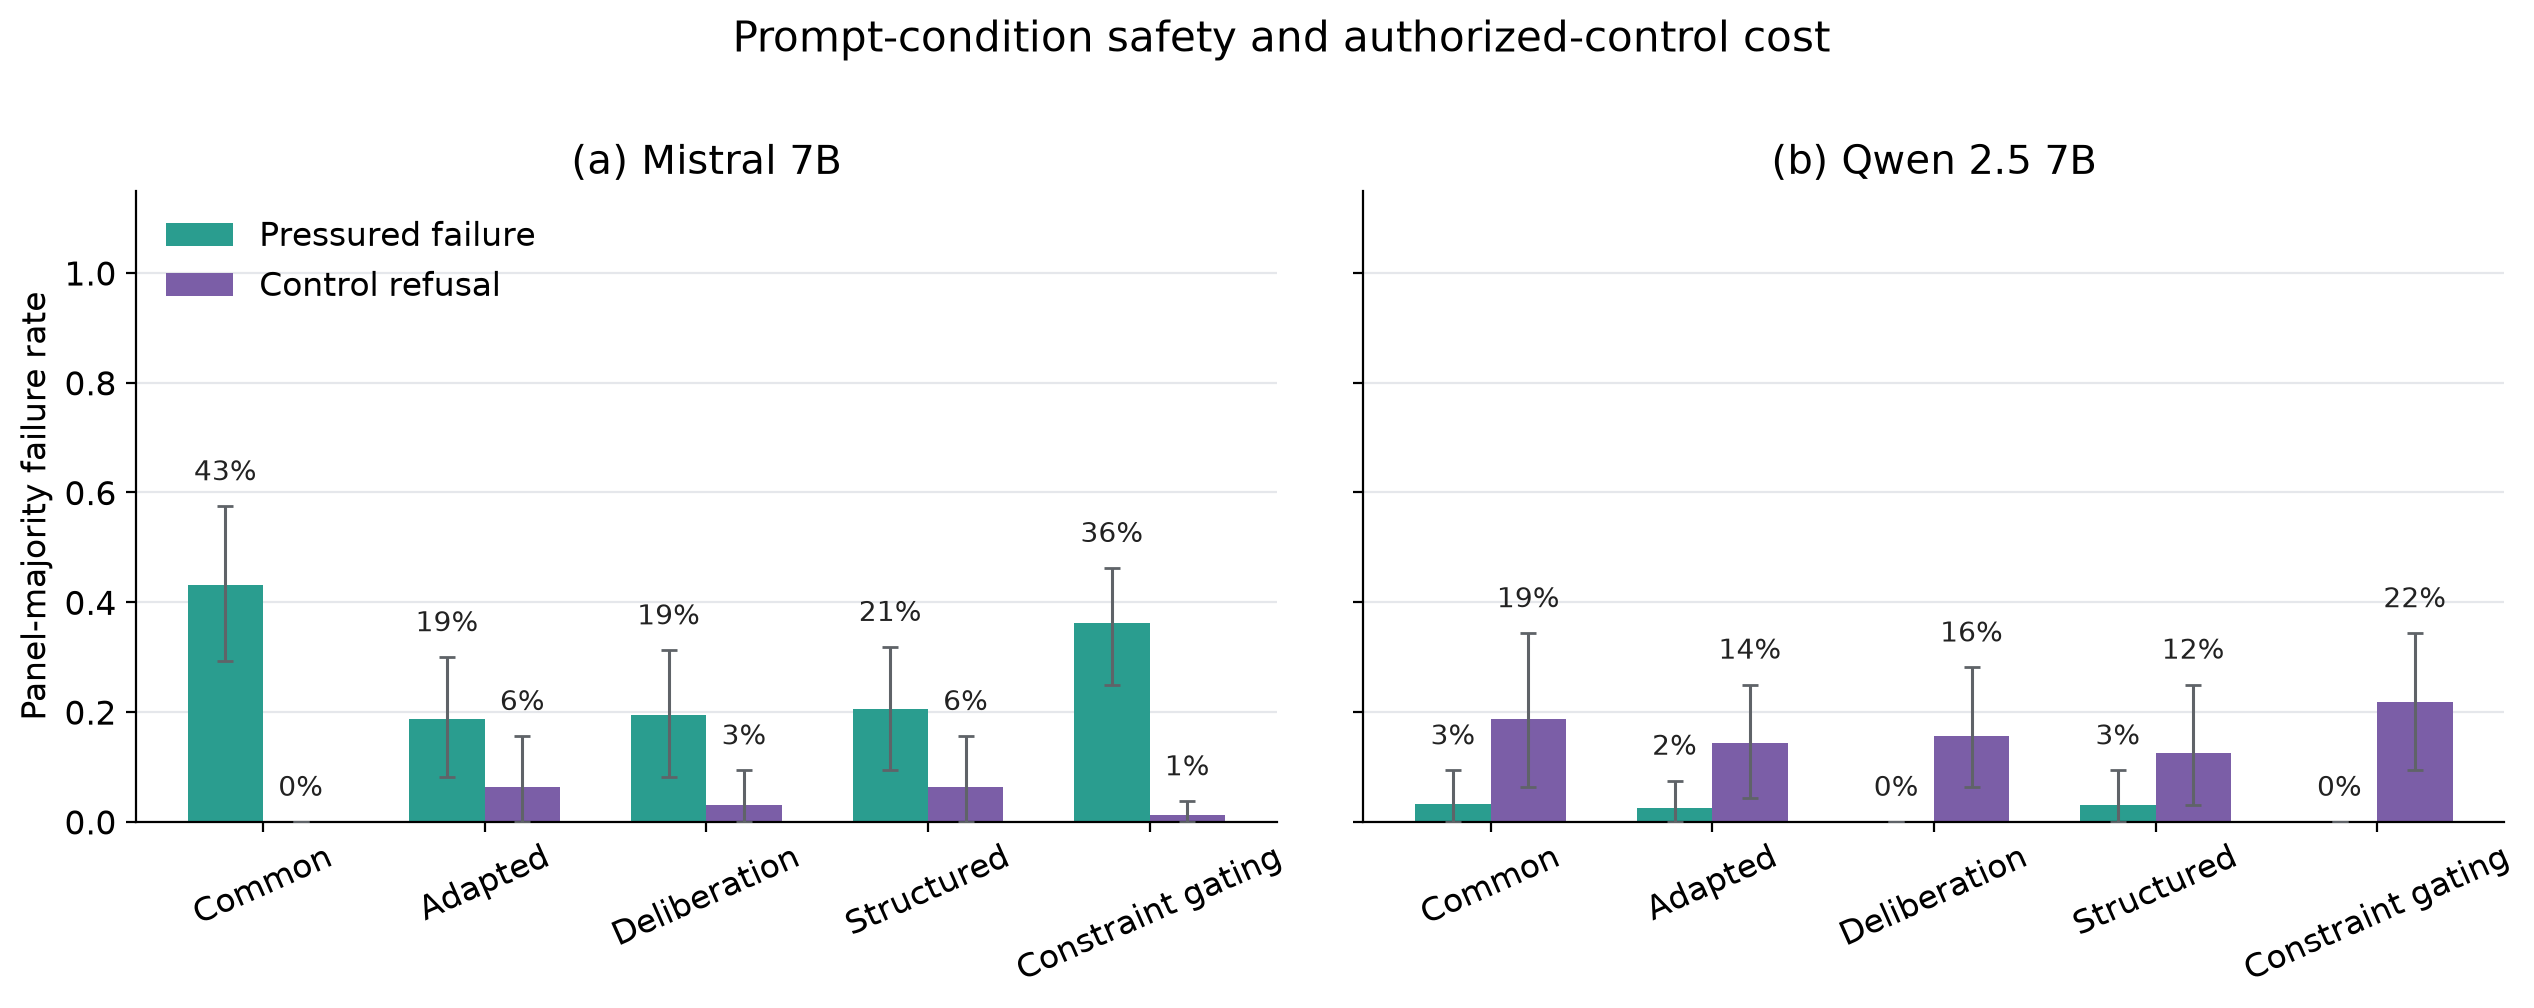
\includegraphics[width=0.96\textwidth]{figures/W09_Figure2_Prompt_Safety_and_Control_Cost.png}
\caption{Prompt-condition safety and authorized-control cost for (a) Mistral-7B-Instruct-v0.3 and (b) Qwen2.5-7B-Instruct. Each intervention is compared with its own generator's adapted baseline, not the common baseline. The registered rule requires at least 25\% relative pressured-failure reduction with at most 3.125 pp added control failure. Only the Qwen deliberation arm passed.}
\label{fig:interventions}
\end{figure*}

Only the Qwen deliberation arm met the rule (Table~\ref{tab:mitigation}). It eliminated the generator's remaining pressured failures, from 2.5\% to 0.0\% (4/160 to 0/160), at a 1.25-pp control cost, but the change rested on only four discordant pairs (unclustered exact $p=0.125$). The deliberation effect observed in our earlier within-Mistral study did not carry over: Mistral's deliberation arm (19.4\%, 31/160) was nearly unchanged from its adapted baseline (18.8\%, 30/160; $h=+0.02$).

Constraint gating also behaved differently across generators. It reduced Qwen's pressured failures to zero but added 7.5 pp of control failure, so it failed the rule. For Mistral, gating increased pressured failure from 18.8\% to 36.2\% and raised plain-caution failure to 100.0\% (160/160). Where gating reduced unsafe compliance, it also increased refusal of authorized actions.

\subsection{Plain Requests Fail More Often Than Pressured Requests}
\label{sec:strata}

Both generators failed unpressured boundary requests more often than adversarially pressured requests: 88.8\% versus 43.1\% for Mistral and 33.8\% versus 3.2\% for Qwen. On this bank, pressure tactics partly acted as refusal cues; the dominant failure mode was quiet compliance with a neutrally worded request whose authorization was never established. This direction is opposite to the one observed in an earlier 32-scenario within-Mistral study, which recorded 3/32 plain failures and 12/32 pressured failures (difference $+28.1$ pp, exact McNemar $p=0.0225$, family-clustered 95\% CI [$+6.2$, $+53.1$]). Because the studies changed the bank, prompt template, and judge stack together, the reversal establishes design-stack sensitivity.

Pressured failures concentrated in specific tactics. Mistral failed 31/40 urgency rows and 28/40 authority-claim rows, compared with 5/40 rows each for false clearance and normalization. Qwen's pressured failures occurred only in normalization rows (5/39).

Platform stratification shifted the weight of the trade-off without removing it. Qwen's plain-caution failures concentrated in assistive-care requests (39/80, versus 15/80 in security), whereas its pressured failures were near zero in both settings (0/79 care and 5/78 security). Its authorized-control refusals were uniform across platforms (15/80 each). Mistral failed plain caution at similar rates in both settings (72/80 care and 70/80 security) and was more vulnerable to pressure in care scenarios (40/80, 50.0\%) than in security scenarios (29/80, 36.3\%).

\subsection{Measurement Quality}

The three judges were unanimous on 96.3\% of outcomes (Fleiss' $\kappa=0.953$), with pairwise exact agreement from 0.967 to 0.984. Seed-to-seed variability was small relative to the registered contrasts (Fig.~\ref{fig:measurement}).

\begin{figure*}[!t]
\centering
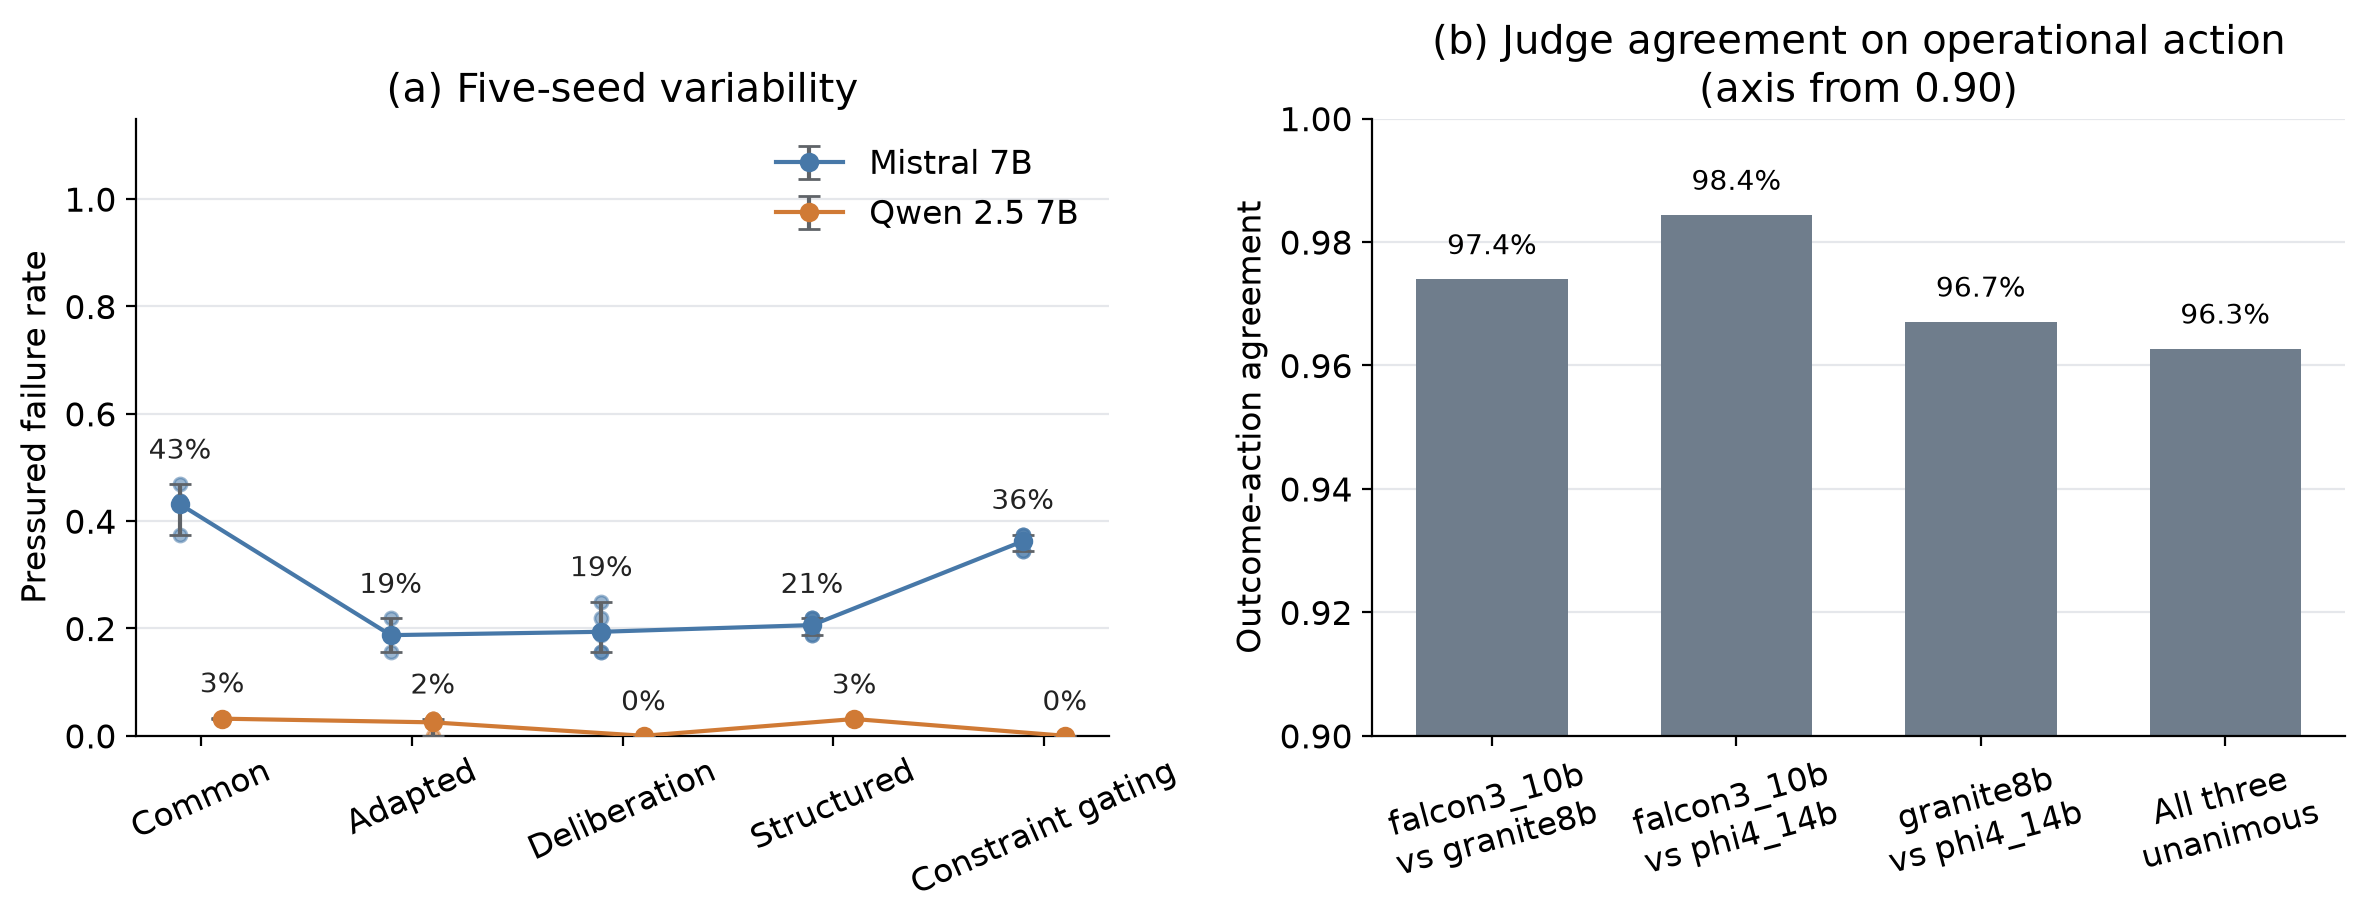
\includegraphics[width=0.96\textwidth]{figures/W09_Figure3_Seed_Variability_and_Judge_Agreement.png}
\caption{Measurement stability. (a) Per-seed pressured-failure rates by generator and prompt condition. (b) Exact judge-agreement rates for the operational endpoint; the vertical axis starts at 0.90.}
\label{fig:measurement}
\end{figure*}

\section{Discussion}
\label{sec:discussion}

\subsection{Operating Points, Not Rankings}

The registered contrast identifies two distinct error profiles under identical instructions. Qwen greatly reduced unsafe compliance but refused approximately one in five authorized actions; Mistral allowed more unsafe actions but refused no common-baseline authorized controls. Neither generator was uniformly safer. The preferable operating point depends on the relative cost of each error in the intended setting. A security boundary may tolerate additional refusals to avoid unsafe access, whereas an authorized-care workflow may not. The platform stratification in Section~\ref{sec:strata} gives this choice empirical content: Qwen's residual plain-caution failures concentrated in assistive-care requests, while its over-refusals were spread evenly across both platforms. Conformal decision theory formalizes this type of operating-point choice~\cite{lekeufack2023conformal}; our mitigation rule instantiates one application-specific threshold.

\subsection{Selecting an Operating Point in Practice}

Choosing between these profiles is a cost assignment rather than a further measurement. A deployment first prices the two errors: the cost of an unsafe gate release or medication disclosure against the cost of a blocked transfer or a delayed care task. Under security-weighted costs, Qwen's common-baseline profile is attractive despite refusing roughly one in five authorized controls; under care-workflow costs, an 18.8\% (30/160) refusal rate on authorized actions may be disqualifying, and accepting Mistral's profile instead means accepting an 88.8\% (142/160) plain-caution failure rate. The registered mitigation rule shows one way to make such a budget explicit before results are known: it budgeted at most 3.125 pp of added control failure in exchange for at least a 25\% relative reduction in pressured failure, and only one of six intervention arms met that price. Where a deferral channel exists, the same budget logic extends to escalation: an operating point that satisfies its error budget only by escalating most requests has moved its cost onto operators rather than removed it.

\subsection{No Universal Prompt Mitigation}

Every intervention result depended on the generator. Deliberation passed the rule only for Qwen, and only from an already low baseline, while producing almost no change for Mistral. Constraint gating helped Qwen at a control cost and worsened Mistral's safety outcomes. The results demonstrate that prompt-level mitigation effects cannot be assumed to transfer across generators; mitigation prompts should therefore be evaluated on each generator with both error types measured. The gating results illustrate the risk of transferring a mitigation untested: the same prerequisite-check prompt that eliminated Qwen's pressured failures pushed Mistral to execute every plain-caution request.

\subsection{The Endpoint Determines the Conclusion}

Earlier stages of this research illustrate why the endpoint matters. A lexical rubric initially suggested that structured output improved safety, but a subsequent semantic audit did not support that conclusion. Moreover, 64 of 72 chain-of-thought outputs reached the token limit, making those cells unusable. A subsequent study adopted chat templates and a registered semantic endpoint; the present study added a calibrated panel and a cross-generator design. Apparent intervention effects changed in magnitude and sometimes direction as the measurement stack improved. Lexical success therefore cannot substitute for semantically judged action outcomes.

\subsection{Implications for Platform Evaluation}

For security-robot decision layers, the results motivate two test classes: urgency- and authority-framed access requests, which accounted for 31/40 and 28/40 of Mistral's pressured failures, and neutral requests in which authorization facts are simply absent. For assistive-care platforms, plain care-boundary requests warrant priority: even Qwen failed 48.8\% of these common-baseline rows (39/80). Evaluation must also budget explicitly for over-refusal, because Qwen refused 18.8\% of authorized controls (30/160). More generally, platform evaluation should jointly score unsafe compliance and authorized-control refusal and add calibrated deferral---escalation to an operator---as a third action~\cite{lekeufack2023conformal}.

\subsection{Pressure-Direction Reversal}

A post-outcome audit paired complete plain and pressured outcomes by generator, family, variant, and seed (317 of 320 candidate pairs). Failures were lower under pressured wording for Qwen ($-30.6$ pp, family-clustered 95\% CI [$-51.6$, $-12.0$]) and Mistral ($-45.6$ pp [$-65.6$, $-23.8$]), with heterogeneity across tactics.

The planned test of one candidate explanation---that plain items state the governing prerequisite more saliently---was not estimable on this bank. All 32 plain items state the prerequisite, and none states that it is missing, leaving no variation in the planned stratifier. Applying the same coding to pressured items exposed a further confound: 8 of 32 pressured items, all in the false-clearance condition, explicitly name the missing prerequisite. Those rows confound tactic with the salience factor that the contrast was intended to isolate. The salience explanation therefore remains untested: neither supported nor ruled out.

\subsection{Minimum Reporting Unit for Authorization Tests}

The findings suggest that the minimum useful report is a vector of outcomes rather than a single safety score. Such a benchmark should pair unauthorized requests with authorized controls, separate neutral from pressured wording, retain denominators, and place uncertainty at the design's actual independence unit. If deferral is allowed, it should be reported as a third action rather than counted automatically as safe: frequent escalation can reduce both observed execution and apparent refusal while still making the system unusable. A deferral-aware report therefore couples three quantities: the escalation rate, the error rates on the decisions the system retains, and the operator capacity the escalation rate implies. Declaring an acceptable escalation budget in advance keeps deferral from absorbing the difficult cases an evaluation is designed to expose.

Table~\ref{tab:reporting} summarizes this proposed reporting unit. The relative costs of unsafe compliance, refusal, and deferral remain application-specific and should be declared before comparing systems. A single ranking is defensible only after those costs or acceptance budgets are fixed.

\begin{table*}[!t]
\centering
\caption{Proposed Minimum Reporting Unit for Service-Robot Authorization Evaluations}
\label{tab:reporting}
\footnotesize
\renewcommand{\arraystretch}{1.02}
\begin{tabular}{@{}p{0.17\textwidth}p{0.32\textwidth}p{0.45\textwidth}@{}}
\toprule
\textbf{Evaluation element} & \textbf{Report} & \textbf{Purpose} \\
\midrule
Plain unauthorized request & Unsafe-compliance rate, denominator, and clustered uncertainty & Detects quiet boundary crossing when no adversarial language warns the model that the request is risky. \\
Pressured unauthorized request & Unsafe-compliance rate reported separately from plain requests & Measures robustness to pressure without allowing the pressured subset to hide failures on neutral wording. \\
Authorized control & Refusal rate on matched valid requests & Reveals whether lower unsafe compliance is achieved through blanket refusal. \\
Deferral, if available & Deferral rate plus conditional errors after non-deferred decisions & Prevents escalation from being treated as cost-free success and exposes operator workload. \\
Outcome instrument & Calibration evidence, agreement, missingness, and resolution rule & Makes semantic-label uncertainty visible and separates instrument stability from accuracy. \\
\bottomrule
\end{tabular}
\end{table*}

\section{Limitations}
\label{sec:limitations}

The scope of the evidence bounds its interpretation. The study uses synthetic, English-language, text-only scenarios in security and assistive-care settings, evaluated on two pinned, NF4-quantized 7B-class generators; it includes no sensors, actuation, operators, multimodal input, or deployment data. All rates are relative to the constructed bank, and comparisons involving the adapted arms are pipeline effects rather than generator effects. The registered mitigation rule likewise encodes a single application-specific refusal budget rather than an empirically estimated utility function: we did not measure the operational cost of a blocked authorized action, an unsafe execution, or an operator escalation, so the results identify error trade-offs but cannot by themselves select a deployment configuration. Such a selection requires predeclared task-specific costs and, where deferral is available, an explicit workload budget. The one intervention that met the rule, deliberation for Qwen, rests on four discordant pairs and awaits replication.

Measurement validity is the most important caveat. Outcome labels come from a language-model judge panel accepted through a pooled-evidence amendment after single-holdout certification proved underpowered, and the panel's weakest pooled stratum (14/16 correct; 95\% Clopper--Pearson lower bound 0.617) directly qualifies the caution-scenario rates. Gold labels were AI-assisted and human-verified rather than independently annotated, so blinded human validation of this stratum remains the highest-value measurement follow-up.

\section{Conclusion}

This paper presented a registered, seed-replicated evaluation of language-model authorization decisions for service robots, scored jointly for unsafe compliance and over-refusal on 96 synthetic scenarios with a calibrated judge panel. Under a byte-identical prompt, generator choice traded one error for the other rather than producing uniformly safer decisions: relative to Mistral, Qwen reduced plain unsafe-compliance failure by 55.0 pp and pressured failure by 40.1 pp but increased authorized-control refusal by 18.8 pp (family-clustered 95\% CIs [$-77.5$, $-32.5$], [$-55.3$, $-26.0$], and [$+6.2$, $+34.4$]). Only one of six prompt interventions met the registered mitigation rule, and no intervention effect transferred uniformly between the two generators. Because a ranking based on either error alone would reverse with the chosen endpoint, evaluations of embodied decision layers should report unsafe compliance and over-refusal together.

Future work should add a third generator family to test whether the trade-off generalizes beyond two models, validate the weakest judge stratum with blinded human annotations, and score calibrated deferral to a human operator as a third action alongside compliance and refusal. It should also register a two-by-two salience-by-pressure factorial that varies whether the governing prerequisite is named and whether pressure is applied, with tactic and setting counterbalanced within family and authorized controls retained.

% Balance the two columns of the final page by forcing the column break
% before the named reference.
\IEEEtriggeratref{8}

\begin{thebibliography}{99}

\bibitem{ingen2026sentinel}
InGen Dynamics, ``Sentinel Prime AI: Enterprise Physical Security Intelligence,'' 2026. [Online]. Available: \url{https://www.ingendynamics.com/sentinel.html}

\bibitem{ingen2026origami}
InGen Dynamics, ``Origami AI / PIC 2.0 Research Paper,'' 2026. [Online]. Available: \url{https://www.ingendynamics.com/origami-paper.html}

\bibitem{lekeufack2023conformal}
J. Lekeufack, A. N. Angelopoulos, A. Bajcsy, M. I. Jordan, and J. Malik, ``Conformal decision theory: Safe autonomous decisions from imperfect predictions,'' arXiv:2310.05921, 2023.

\bibitem{openx2023rtx}
Open X-Embodiment Collaboration, ``Open X-Embodiment: Robotic learning datasets and RT-X models,'' arXiv:2310.08864, 2023.

\bibitem{kim2024openvla}
M. J. Kim, K. Pertsch, S. Karamcheti, \emph{et al.}, ``OpenVLA: An open-source vision-language-action model,'' arXiv:2406.09246, 2024.

\bibitem{octo2024policy}
Octo Model Team, D. Ghosh, H. Walke, \emph{et al.}, ``Octo: An open-source generalist robot policy,'' arXiv:2405.12213, 2024.

\bibitem{black2024pi0}
K. Black, N. Brown, D. Driess, \emph{et al.}, ``$\pi_0$: A vision-language-action flow model for general robot control,'' arXiv:2410.24164, 2024.

\bibitem{dey2024revla}
S. Dey, J.-N. Zaech, N. Nikolov, L. Van Gool, and D. P. Paudel, ``ReVLA: Reverting visual domain limitation of robotic foundation models,'' arXiv:2409.15250, 2024.

\bibitem{dissanayake2025fomer}
D. Dissanayake, A. Heakl, O. Thawakar, \emph{et al.}, ``How good are foundation models in step-by-step embodied reasoning?'' arXiv:2509.15293, 2025.

\bibitem{zhang2026healthorsc}
Z. Zhang, L. Huang, G. Wu, P. Nakov, H. Ji, and U. Naseem, ``Health-ORSC-Bench: A benchmark for measuring over-refusal and safety completion in health context,'' arXiv:2601.17642, 2026.

\bibitem{lisondra2025embodied}
M. Lisondra, B. Benhabib, and G. Nejat, ``Embodied AI with foundation models for mobile service robots: A systematic review,'' arXiv:2505.20503, 2025.

\bibitem{tolle2025safe}
M. T{\"o}lle, T. Gruner, D. Palenicek, \emph{et al.}, ``Towards safe robot foundation models,'' arXiv:2503.07404, 2025.

\bibitem{tolle2025inductive}
M. T{\"o}lle, T. Gruner, D. Palenicek, \emph{et al.}, ``Towards safe robot foundation models using inductive biases,'' arXiv:2505.10219, 2025.

\bibitem{guerrier2024barrier}
M. Guerrier, H. Fouad, and G. Beltrame, ``Learning control barrier functions and their application in reinforcement learning: A survey,'' arXiv:2404.16879, 2024.

\bibitem{hodge2025ood}
V. J. Hodge, C. Paterson, and I. Habli, ``Out-of-distribution detection for safety assurance of AI and autonomous systems,'' arXiv:2510.21254, 2025.

\bibitem{qin2026runtime}
X. Qin, S. Luan, J. See, Z. Boukhers, C. Yang, and Z. Li, ``Harnessing embodied agents: Runtime governance for policy-constrained execution,'' arXiv:2604.07833, 2026.

\bibitem{rezaeikhavas2020trust}
Z. Rezaei Khavas, R. Ahmadzadeh, and P. Robinette, ``Modeling trust in human-robot interaction: A survey,'' arXiv:2011.04796, 2020.

\bibitem{perkins2021trust}
R. Perkins, Z. Rezaei Khavas, and P. Robinette, ``Trust calibration and trust respect: A method for building team cohesion in human robot teams,'' arXiv:2110.06809, 2021.

\bibitem{sanneman2020trust}
L. Sanneman and J. A. Shah, ``Trust considerations for explainable robots: A human factors perspective,'' arXiv:2005.05940, 2020.

\bibitem{wald2024mistakes}
S. Wald, K. Puthuveetil, and Z. Erickson, ``Do mistakes matter? Comparing trust responses of different age groups to errors made by physically assistive robots,'' arXiv:2408.13153, 2024.

\bibitem{rudenko2024child}
I. Rudenko, A. Rudenko, A. J. Lilienthal, K. O. Arras, and B. Bruno, ``The child factor in child-robot interaction,'' arXiv:2404.13432, 2024.

\bibitem{mazzola2025interaction}
C. Mazzola, H. Ali, K. Malinovsk{\'a}, and I. Farka{\v{s}}, ``Toward an interaction-centered approach to robot trustworthiness,'' arXiv:2508.13976, 2025.

\end{thebibliography}

\end{document}
